% Four-step prompt-evaluation loop for Ch22 ("Evaluating a Prompt") — the Vol 3 eval pair, prompt side.
% Standalone TikZ; compiled by `book-scaffold build-figures` via pdflatex -> pdftocairo -> SVG.
% Two fixed preconditions (define criteria, build test cases) gate entry to a two-step iterate/grade
% cycle: (3) iterate with tooling (prompt improver drafts; Console eval measures) -> (4) grade by
% reliability-per-effort -> back to iterate. The whole cycle loops back to the preconditions.
\documentclass[tikz,border=4mm]{standalone}
\usepackage{tikz}
\usetikzlibrary{positioning, arrows.meta, calc, decorations.pathreplacing}

\begin{document}
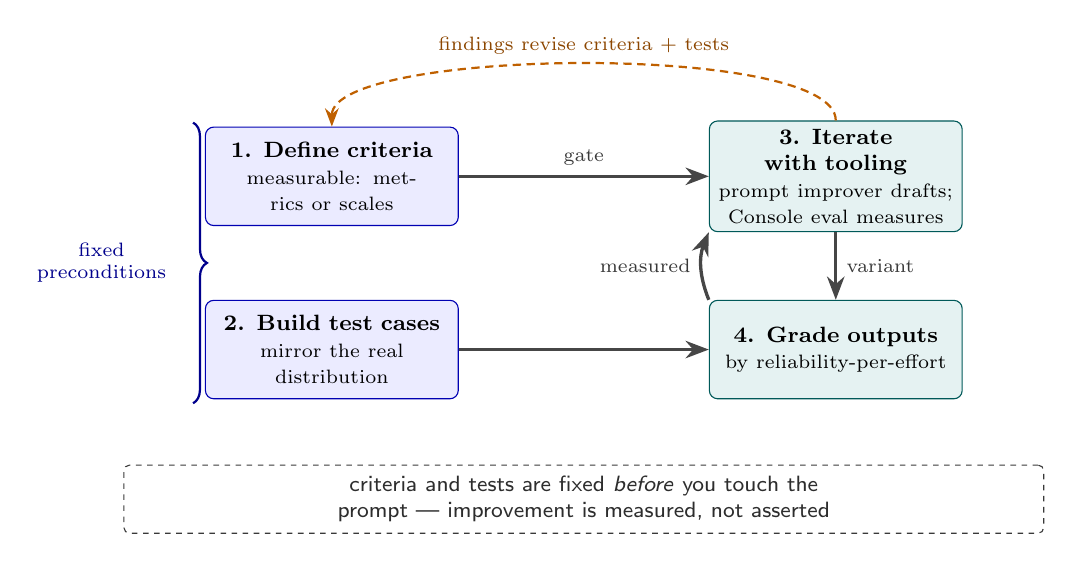
\begin{tikzpicture}[
  font=\sffamily,
  pre/.style={draw=blue!70!black, fill=blue!8, rounded corners=3pt, align=center,
    text width=3.0cm, minimum height=1.25cm, inner sep=3pt, font=\footnotesize},
  cyc/.style={draw=teal!70!black, fill=teal!10, rounded corners=3pt, align=center,
    text width=3.0cm, minimum height=1.25cm, inner sep=3pt, font=\footnotesize},
  flow/.style={-Stealth, very thick, draw=gray!55!black},
  back/.style={-Stealth, thick, draw=orange!75!black, dash pattern=on 3pt off 2pt}
]

% --- the two FIXED preconditions (gate), stacked at left ---
\node[pre] (p1) at (0,1.1)  {\textbf{1. Define criteria}\\{\scriptsize measurable: metrics or scales}};
\node[pre] (p2) at (0,-1.1) {\textbf{2. Build test cases}\\{\scriptsize mirror the real distribution}};

% brace marking the two as the fixed precondition gate
\draw[decorate, decoration={brace, amplitude=5pt, mirror}, draw=blue!55!black, thick]
  ($(p2.south west)+(-0.15,-0.05)$) -- ($(p1.north west)+(-0.15,0.05)$)
  node[midway, left=6pt, align=center, font=\scriptsize, text=blue!55!black]
  {fixed\\preconditions};

% --- the two-step iterate/grade CYCLE at right ---
\node[cyc] (c3) at (6.4,1.1)  {\textbf{3. Iterate with tooling}\\{\scriptsize prompt improver drafts; Console eval measures}};
\node[cyc] (c4) at (6.4,-1.1) {\textbf{4. Grade outputs}\\{\scriptsize by reliability-per-effort}};

% preconditions gate entry into the cycle
\draw[flow] (p1.east) -- (c3.west) node[midway, above, font=\scriptsize, text=gray!45!black] {gate};
\draw[flow] (p2.east) -- (c4.west);

% the inner cycle: iterate -> grade -> iterate
\draw[flow] (c3.south) -- (c4.north) node[midway, right, font=\scriptsize, text=gray!45!black] {variant};
\draw[flow] (c4.north west) to[bend left=22] node[midway, left, font=\scriptsize, text=gray!45!black] {measured} (c3.south west);

% dashed return: the loop revises the criteria/tests
\draw[back] (c3.north) .. controls +(0,1.0) and +(0,1.0) .. (p1.north)
  node[midway, above, font=\scriptsize, text=orange!55!black] {findings revise criteria + tests};

% caption strip beneath
\node[draw=gray!45!black, dash pattern=on 2pt off 2pt, rounded corners=2pt, align=center,
  text width=11.4cm, inner sep=4pt, font=\sffamily\footnotesize, text=gray!35!black]
  at (3.2,-3.0) {criteria and tests are fixed \emph{before} you touch the prompt --- improvement is measured, not asserted};

\end{tikzpicture}
\end{document}
